\documentclass{standalone}
\usepackage{tikz}
\usetikzlibrary{patterns, positioning}

\begin{document}
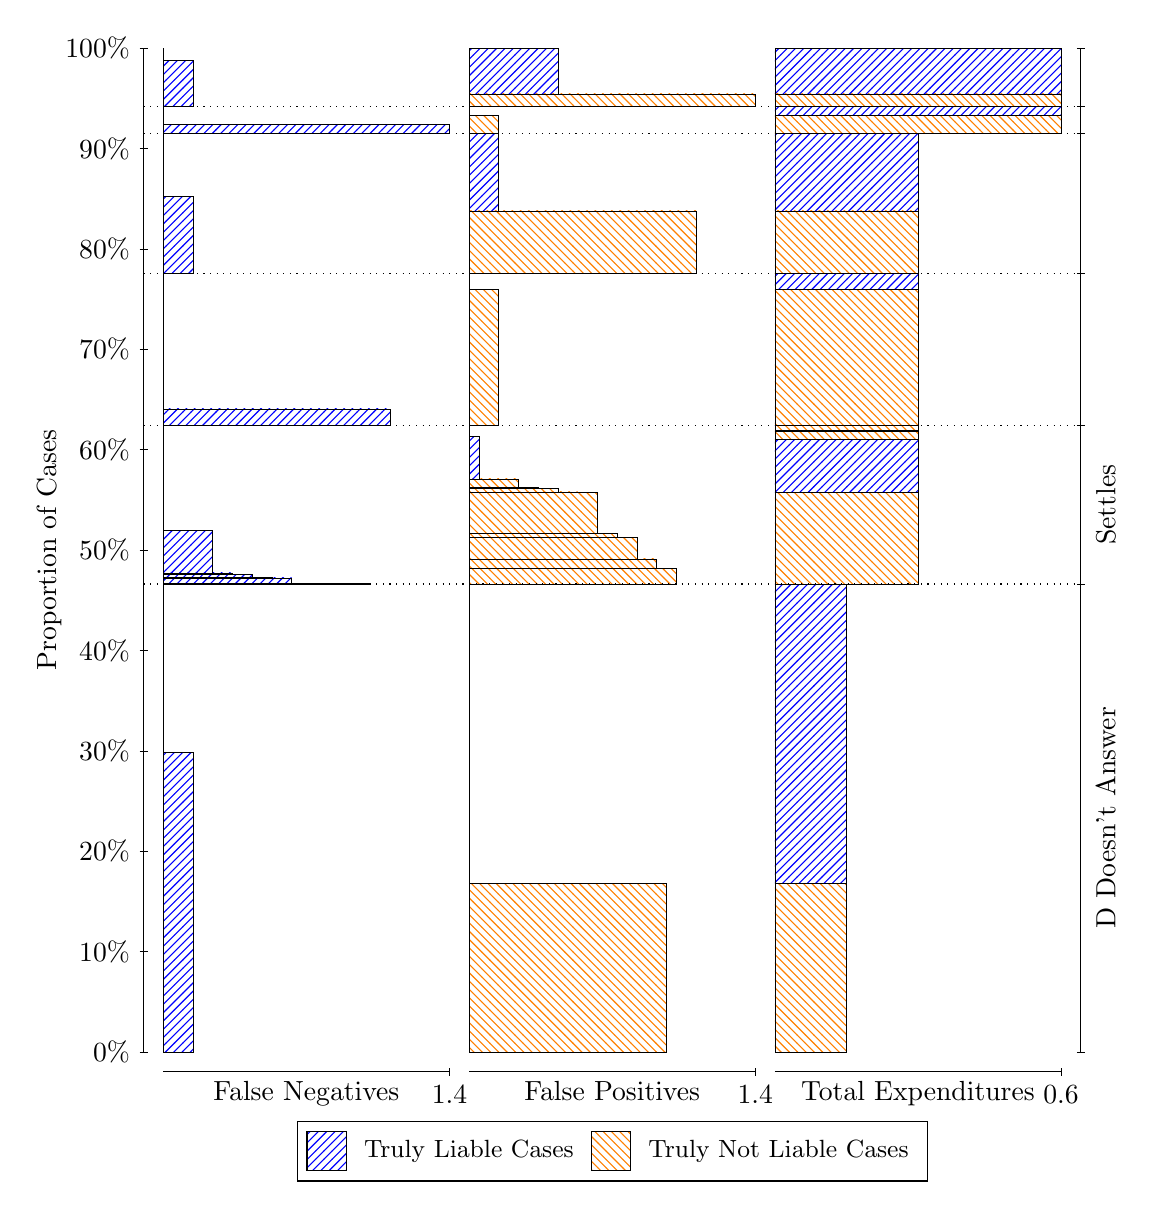
\begin{tikzpicture}
\draw[black, very thin] (1.5,1.75) -- (1.5,14.5);
\node[rotate=90, anchor=center] at (0.3, 8.125) {Proportion of Cases};
\draw[black, very thin] (1.45,1.75) -- (1.55,1.75);
\node[anchor=east] at (1.45, 1.75) {0\%};
\draw[black, very thin] (1.45,3.025) -- (1.55,3.025);
\node[anchor=east] at (1.45, 3.025) {10\%};
\draw[black, very thin] (1.45,4.3) -- (1.55,4.3);
\node[anchor=east] at (1.45, 4.3) {20\%};
\draw[black, very thin] (1.45,5.575) -- (1.55,5.575);
\node[anchor=east] at (1.45, 5.575) {30\%};
\draw[black, very thin] (1.45,6.85) -- (1.55,6.85);
\node[anchor=east] at (1.45, 6.85) {40\%};
\draw[black, very thin] (1.45,8.125) -- (1.55,8.125);
\node[anchor=east] at (1.45, 8.125) {50\%};
\draw[black, very thin] (1.45,9.4) -- (1.55,9.4);
\node[anchor=east] at (1.45, 9.4) {60\%};
\draw[black, very thin] (1.45,10.675) -- (1.55,10.675);
\node[anchor=east] at (1.45, 10.675) {70\%};
\draw[black, very thin] (1.45,11.95) -- (1.55,11.95);
\node[anchor=east] at (1.45, 11.95) {80\%};
\draw[black, very thin] (1.45,13.225) -- (1.55,13.225);
\node[anchor=east] at (1.45, 13.225) {90\%};
\draw[black, very thin] (1.45,14.5) -- (1.55,14.5);
\node[anchor=east] at (1.45, 14.5) {100\%};

\draw[black, very thin] (13.4,1.75) -- (13.4,14.5);
\draw[black, very thin] (13.35,1.75) -- (13.45,1.75);
\node[anchor=west] at (13.35, 1.75) {};
\draw[black, very thin] (13.35,7.6932) -- (13.45,7.6932);
\node[anchor=west] at (13.35, 7.6932) {};
\draw[black, very thin] (13.35,9.7096) -- (13.45,9.7096);
\node[anchor=west] at (13.35, 9.7096) {};
\draw[black, very thin] (13.35,11.639) -- (13.45,11.639);
\node[anchor=west] at (13.35, 11.639) {};
\draw[black, very thin] (13.35,13.412) -- (13.45,13.412);
\node[anchor=west] at (13.35, 13.412) {};
\draw[black, very thin] (13.35,13.762) -- (13.45,13.762);
\node[anchor=west] at (13.35, 13.762) {};
\draw[black, very thin] (13.35,14.5) -- (13.45,14.5);
\node[anchor=west] at (13.35, 14.5) {};

\draw[black, very thin, pattern color=blue, pattern=north east lines] (1.75,1.75) rectangle (2.1259,5.5545);
\draw[black, very thin, pattern color=orange, pattern=north west lines] (1.75,5.5545) rectangle (1.75,7.6932);
\draw[black, very thin, pattern color=blue, pattern=north east lines] (1.75,7.6932) rectangle (4.381,7.6993);
\draw[black, very thin, pattern color=blue, pattern=north east lines] (1.75,7.6993) rectangle (4.1305,7.7001);
\draw[black, very thin, pattern color=blue, pattern=north east lines] (1.75,7.7001) rectangle (3.8799,7.703);
\draw[black, very thin, pattern color=blue, pattern=north east lines] (1.75,7.703) rectangle (3.6293,7.7036);
\draw[black, very thin, pattern color=blue, pattern=north east lines] (1.75,7.7036) rectangle (3.3787,7.7712);
\draw[black, very thin, pattern color=blue, pattern=north east lines] (1.75,7.7712) rectangle (3.1282,7.7774);
\draw[black, very thin, pattern color=blue, pattern=north east lines] (1.75,7.7774) rectangle (2.8776,7.8194);
\draw[black, very thin, pattern color=blue, pattern=north east lines] (1.75,7.8194) rectangle (2.627,7.8355);
\draw[black, very thin, pattern color=blue, pattern=north east lines] (1.75,7.8355) rectangle (2.3764,8.3746);
\draw[black, very thin, pattern color=orange, pattern=north west lines] (1.75,8.3746) rectangle (1.75,9.7096);
\draw[black, very thin, pattern color=blue, pattern=north east lines] (1.75,9.7096) rectangle (4.6316,9.9171);
\draw[black, very thin, pattern color=orange, pattern=north west lines] (1.75,9.9171) rectangle (1.75,11.639);
\draw[black, very thin, pattern color=blue, pattern=north east lines] (1.75,11.639) rectangle (2.1259,12.62);
\draw[black, very thin, pattern color=orange, pattern=north west lines] (1.75,12.62) rectangle (1.75,13.412);
\draw[black, very thin, pattern color=blue, pattern=north east lines] (1.75,13.412) rectangle (5.3833,13.529);
\draw[black, very thin, pattern color=orange, pattern=north west lines] (1.75,13.529) rectangle (1.75,13.762);
\draw[black, very thin, pattern color=blue, pattern=north east lines] (1.75,13.762) rectangle (2.1259,14.345);
\draw[black, very thin, pattern color=orange, pattern=north west lines] (1.75,14.345) rectangle (1.75,14.5);
\draw[black, very thin, pattern color=orange, pattern=north west lines] (5.6333,1.75) rectangle (8.1391,3.8887);
\draw[black, very thin, pattern color=blue, pattern=north east lines] (5.6333,3.8887) rectangle (5.6333,7.6932);
\draw[black, very thin, pattern color=orange, pattern=north west lines] (5.6333,7.6932) rectangle (8.2644,7.8958);
\draw[black, very thin, pattern color=orange, pattern=north west lines] (5.6333,7.8958) rectangle (8.0138,8.0122);
\draw[black, very thin, pattern color=orange, pattern=north west lines] (5.6333,8.0122) rectangle (7.7632,8.2888);
\draw[black, very thin, pattern color=orange, pattern=north west lines] (5.6333,8.2888) rectangle (7.5126,8.3318);
\draw[black, very thin, pattern color=orange, pattern=north west lines] (5.6333,8.3318) rectangle (7.2621,8.852);
\draw[black, very thin, pattern color=orange, pattern=north west lines] (5.6333,8.852) rectangle (7.0115,8.8582);
\draw[black, very thin, pattern color=orange, pattern=north west lines] (5.6333,8.8582) rectangle (7.0115,8.8617);
\draw[black, very thin, pattern color=orange, pattern=north west lines] (5.6333,8.8617) rectangle (6.7609,8.9097);
\draw[black, very thin, pattern color=orange, pattern=north west lines] (5.6333,8.9097) rectangle (6.5103,8.9221);
\draw[black, very thin, pattern color=orange, pattern=north west lines] (5.6333,8.9221) rectangle (6.2598,9.0282);
\draw[black, very thin, pattern color=blue, pattern=north east lines] (5.6333,9.0282) rectangle (5.7586,9.5673);
\draw[black, very thin, pattern color=blue, pattern=north east lines] (5.6333,9.5673) rectangle (5.6333,9.7096);
\draw[black, very thin, pattern color=orange, pattern=north west lines] (5.6333,9.7096) rectangle (6.0092,11.432);
\draw[black, very thin, pattern color=blue, pattern=north east lines] (5.6333,11.432) rectangle (5.6333,11.639);
\draw[black, very thin, pattern color=orange, pattern=north west lines] (5.6333,11.639) rectangle (8.5149,12.431);
\draw[black, very thin, pattern color=blue, pattern=north east lines] (5.6333,12.431) rectangle (6.0092,13.412);
\draw[black, very thin, pattern color=orange, pattern=north west lines] (5.6333,13.412) rectangle (6.0092,13.645);
\draw[black, very thin, pattern color=blue, pattern=north east lines] (5.6333,13.645) rectangle (5.6333,13.762);
\draw[black, very thin, pattern color=orange, pattern=north west lines] (5.6333,13.762) rectangle (9.2667,13.917);
\draw[black, very thin, pattern color=blue, pattern=north east lines] (5.6333,13.917) rectangle (6.7609,14.5);
\draw[black, very thin, pattern color=orange, pattern=north west lines] (9.5167,1.75) rectangle (10.425,3.8887);
\draw[black, very thin, pattern color=blue, pattern=north east lines] (9.5167,3.8887) rectangle (10.425,7.6932);
\draw[black, very thin, pattern color=orange, pattern=north west lines] (9.5167,7.6932) rectangle (11.333,8.8582);
\draw[black, very thin, pattern color=blue, pattern=north east lines] (9.5167,8.8582) rectangle (11.333,9.5297);
\draw[black, very thin, pattern color=orange, pattern=north west lines] (9.5167,9.5297) rectangle (11.333,9.6357);
\draw[black, very thin, pattern color=blue, pattern=north east lines] (9.5167,9.6357) rectangle (11.333,9.6418);
\draw[black, very thin, pattern color=orange, pattern=north west lines] (9.5167,9.6418) rectangle (11.333,9.7057);
\draw[black, very thin, pattern color=blue, pattern=north east lines] (9.5167,9.7057) rectangle (11.333,9.7096);
\draw[black, very thin, pattern color=orange, pattern=north west lines] (9.5167,9.7096) rectangle (11.333,11.432);
\draw[black, very thin, pattern color=blue, pattern=north east lines] (9.5167,11.432) rectangle (11.333,11.639);
\draw[black, very thin, pattern color=orange, pattern=north west lines] (9.5167,11.639) rectangle (11.333,12.431);
\draw[black, very thin, pattern color=blue, pattern=north east lines] (9.5167,12.431) rectangle (11.333,13.412);
\draw[black, very thin, pattern color=orange, pattern=north west lines] (9.5167,13.412) rectangle (13.15,13.645);
\draw[black, very thin, pattern color=blue, pattern=north east lines] (9.5167,13.645) rectangle (13.15,13.762);
\draw[black, very thin, pattern color=orange, pattern=north west lines] (9.5167,13.762) rectangle (13.15,13.917);
\draw[black, very thin, pattern color=blue, pattern=north east lines] (9.5167,13.917) rectangle (13.15,14.5);
\draw[black, dotted] (1.5,7.6932) -- (13.4,7.6932);
\draw[black, dotted] (1.5,9.7096) -- (13.4,9.7096);
\draw[black, dotted] (1.5,11.639) -- (13.4,11.639);
\draw[black, dotted] (1.5,13.412) -- (13.4,13.412);
\draw[black, dotted] (1.5,13.762) -- (13.4,13.762);
\draw[black, very thin] (1.75,1.5) -- (5.3833,1.5);
\node[anchor=north] at (3.5667, 1.5) {False Negatives};
\draw[black, very thin] (5.3833,1.45) -- (5.3833,1.55);
\node[anchor=north] at (5.3833, 1.45) {1.4};

\draw[black, very thin] (5.6333,1.5) -- (9.2667,1.5);
\node[anchor=north] at (7.45, 1.5) {False Positives};
\draw[black, very thin] (9.2667,1.45) -- (9.2667,1.55);
\node[anchor=north] at (9.2667, 1.45) {1.4};

\draw[black, very thin] (9.5167,1.5) -- (13.15,1.5);
\node[anchor=north] at (11.333, 1.5) {Total Expenditures};
\draw[black, very thin] (13.15,1.45) -- (13.15,1.55);
\node[anchor=north] at (13.15, 1.45) {0.6};

\node[black, centered, rotate=90] at (13.72, 4.7216) {D Doesn't Answer};
\node[black, centered, rotate=90] at (13.72, 8.7014) {Settles};





\draw (7.449999999999999,1.5) node[draw=none] (baseCoordinate) {};
\begin{scope}[align=center]
        \matrix[scale=0.5, draw=black, below=0.5cm of baseCoordinate, nodes={draw}, column sep=0.1cm]{
            \node[rectangle, draw, minimum width=0.5cm, minimum height=0.5cm, pattern=north east lines, pattern color=blue] {}; &
            \node[draw=none, font=\small] (B) {Truly Liable Cases}; &
            \node[rectangle, draw, minimum width=0.5cm, minimum height=0.5cm, pattern=north west lines, pattern color=orange] {}; &
            \node[draw=none, font=\small] (B) {Truly Not Liable Cases}; \\
            };
\end{scope}

\end{tikzpicture}
\end{document}